\documentclass[10pt]{article}
\usepackage[margin=0.5in]{geometry} % Set the margins to 0.5 inches
\usepackage{amssymb, amsmath, amsthm, amsfonts}
\usepackage{thmtools, mathtools, mathrsfs, dsfont}
\usepackage{bbm}
\usepackage[super,sort&compress]{natbib}%\bibliographystyle{abbrvnat}
%\usepackage[square,numbers]{natbib} \bibliographystyle{abbrvnat}
\usepackage{lipsum} % For placeholder text (remove if not needed)
\usepackage{setspace} % For line spacing, if needed
%\onehalfspacing % Uncomment for 1.5 line spacing
\usepackage[pdftex]{graphicx}  %remove demo option in your document
\graphicspath{{figures}}
\usepackage[colorlinks]{hyperref}
\bibliographystyle{apj_w_etal_3auth}

\usepackage{paralist}

\renewenvironment{thebibliography}[1]{%
\textsc{\textbf{References:}}
\let\par\relax\let\newblock\relax%
\inparaitem[{[}1{]}]}{\endinparaitem}

\newtheorem{theorem}{Theorem}
\newcommand{\reals}{\mathbb{R}}

\begin{document}

%TODO: f is Lipschitz and structural stability, normal hyperbolicity etc

%\title{RNNs can approximate multistable dynamical systems on an infinite time horizon}
\title{A taxonomy for errors for models of neural computation}
%\author{}
%\date{\today}
%\maketitle

\begin{center}
\Large{RNNs can approximate multistable dynamical systems on an infinite time horizon}
\end{center}

%\section*{Abstract}
\noindent
Deep-learning techniques used for modeling neural dynamics are commonly based on universal dynamics approximators \citep{durstewitz2023reconstructing}.
There is an extensive list of results about universal approximation results of RNNs in the space of dynamical systems \citep{li2022approximation,jiang2023brief}.
These results about the universality of RNNs for dynamical systems can be divided into two groups.
 The first group of results considers finite time horizon approximation results.
  The problem with these is that beyond this finite time horizon, there is no guarantee that the approximation will behave similar to the target system.
   Two main kinds of divergence between target and approximation can be distinguished.
   The first occurs for trajectories that originate in the region where solutions for the target converge to attractor $A_i$ and solutions for the approximation converge to attractor $A_j$ (which is at least epsilon removed from attractor $A_i$, see Fig.~\ref{fig:figure}A). 
   The type of error typically considered in the literature comprises the maximal divergence of trajectories up to a finite time interval (Fig.~\ref{fig:figure}B).
   The second type of divergence occurs for stable limit cycles. If there is (an arbitrarily small) mismatch in periods between target and approximation up to time $T$, the trajectories of the two will diverge after $T$ (Fig.~\ref{fig:figure}C).
  The second group of results considers approximation for dynamical systems with a unique globally stable attractor, typically in the form of the echo state property \citep{jaeger2001echo}.
   The problem with this group is obvious: they leave out a great deal of dynamical systems from the target space that might be relevant for the modelling of neural computation \citep{wong2006timeintegration,mante2013context} (see Fig.~\ref{fig:figure}D).
    This means that the types of dynamics that they can approximate is not rich enough for the richness that brain dynamics are believed to exhibit (Fig.~\ref{fig:figure}D). 
Finally, these results fully describe the types of errors between target dynamics and its approximations.
  First, what we refer to as \emph{basin-type error}, describes trajectories (of the target and approximation starting at the same initial value) diverging to different attractors as described above.
  Second, what we refer to as \emph{trajectory-type error}, occurs when trajectories diverge but then converge to nearby attractors. %include flowtype_error into figure? 
  Third, what we refer to as \emph{period-type error}, occurs when a mismatch between the target and approximation targets exist.
  
We will now shortly state of the main theoretical result.
We consider a compact $X$ on which we measure the difference between the target and our approximation.
First, of all, we compare trajectories through the uniform norm over time (given the same initial starting point):
\begin{equation}
\|\varphi(t,x_0)-\hat \varphi(t,x_0)\|_\infty = \sup_t|\varphi(t,x_0)-\hat \varphi(t,x_0)|.
\end{equation}
Then, we look at the proportion of trajectories which diverge more than $\epsilon$ over all initial points in the compact state space $X$ (similar to the metrics in \citep{hammer2000approximation} and \citep{hanson2021learning}):
\begin{equation}
%\|\varphi-\hat \varphi\|_\epsilon \coloneqq \frac{1}{\vol X}\mathbb{E}\left[ \int_{x_0\in X}   \mathds{1}[\|\varphi(t,x_0)-\hat \varphi(t,x_0)\|_\infty>\epsilon]\right],
\|\varphi-\hat \varphi\|_\epsilon \coloneqq  \mathbb{P}\left(\|\varphi(\cdot,x_0)-\hat \varphi(\cdot,x_0)\|_\infty>\epsilon\right).
\end{equation}
%where $\mathds{1}[\cdot]$ is the indicator function. 

\vspace{-.3cm}
\begin{theorem}
Let $D$ be an open subset of $\mathbb{R}^n$, $f\colon D \to \mathbb{R}^m$ be a $C^1$-mapping, and $I$ be a compact subset of $D$ such that any solution $x(t)$ with initial value $x(0) \in I$ of an ordinary differential equation $\dot{x} = f(x)$ is defined for $t\in\reals_{+}$ and $x(t)$ is included in $I$ and hence defines a flow $\varphi(\cdot, \cdot)$.
 Then, for an arbitrary $\epsilon, \delta > 0$, there exist an multilayer Perceptron (MLP) recurrent neural network 
 \begin{equation}
\dot x = \hat f(x) = \sigma(A\sigma(Bx+b)+a)
\end{equation}
%such that for a solution $\hat \varphi(t,x_0)$ satisfying Eq~\ref{eq:5} with initial state $x_0$ of the network
such that its flow $\hat \varphi$ satisfies $\|\varphi-\hat \varphi\|_\epsilon < \delta.$
\end{theorem}

Finally, normally hyperbolic continuous attractors can be approximated by covering them with a gird stable fixed points or limit cycles that are at most $\epsilon$ far apart \citep{Sagodi2024a}.

\begin{figure}[tbhp]
  \centering
  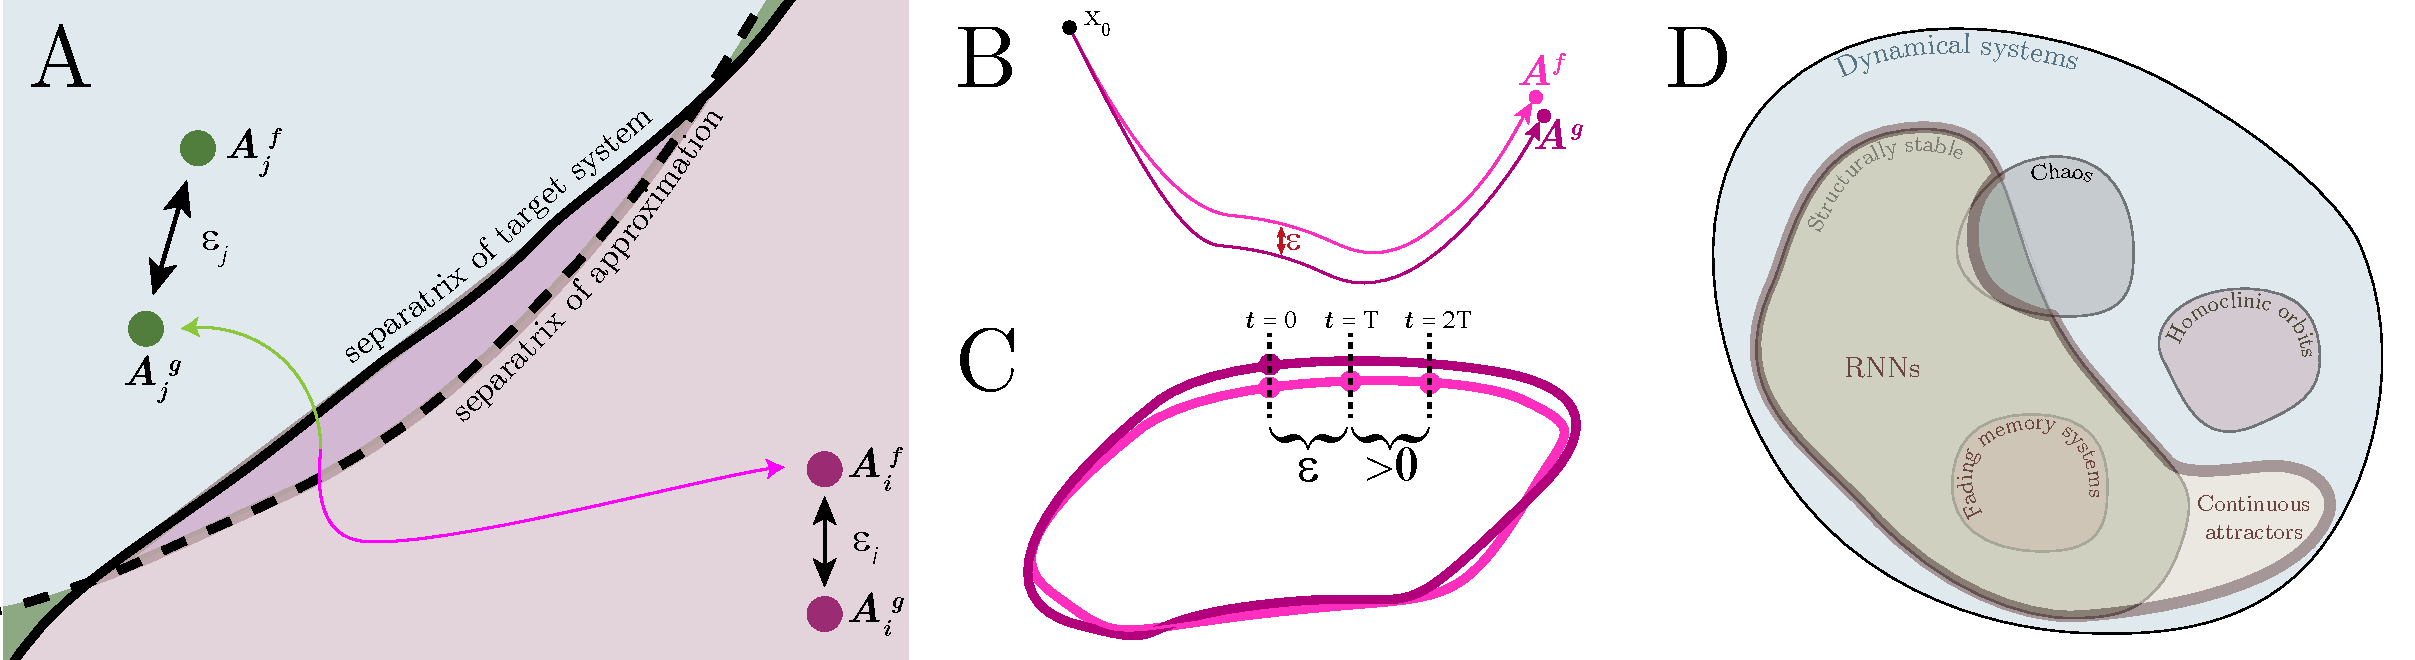
\includegraphics[width=\textwidth]{icmns2025_figure}
  \caption{(A) 	A mismatching pair of separatrices between attractors $A_i$ and $A_j$.
  		(B) Divergence of orbits at limit cycles after $T$.
  		(C) RNNs are dense in the space of Lipschitz dynamical systems.
  }\label{fig:figure}
\end{figure}

%\printbibliography
\bibliography{../all_ref.bib,../catniplab.bib}

\end{document}
